\newcommand{\iso}{[C$_3$H$_3$]$^+$ }
\newcommand{\isoD}{[C$_3$D$_3$]$^+$ }
\newcommand{\cyc}{c-C$_3$H$_3^+$ }
\newcommand{\cycD}{c-C$_3$D$_3^+$ }
\newcommand{\lin}{H$_2$C$_3$H$^+$ }
\newcommand{\linD}{D$_2$C$_3$D$^+$ }
\newcommand{\ison}{[C$_3$H$_3$]$^+$}
\newcommand{\isoDn}{[C$_3$D$_3$]$^+$}
\newcommand{\cycn}{c-C$_3$H$_3^+$}
\newcommand{\cycDn}{c-C$_3$D$_3^+$}
\newcommand{\linn}{H$_2$C$_3$H$^+$}
\newcommand{\linDn}{D$_2$C$_3$D$^+$}

\section*{Abstract}
Gas phase vibrational spectra of \iso isomers and their fully deuterated isotopologues 
measured in a cryogenic 22-pole ion trap are presented. The widely tunable free electron 
laser for infrared experiments, FELIX, was employed to cover the frequency range 
500-2400~\wn, complemented with an OPO/OPA system covering 2800-3400~\wn. 
Spectral assignments for both the linear and cyclic isomeric form 
(\lin and \cycn, respectively) are made based on various high-level 
computational studies. The effect of ion source conditions and 
different precursors (allene and propargyl chloride) for the preferential 
production of a specific isomer is discussed. 
The perturbation of the vibrational band position due to complexation with Neon in the recorded infrared-predissociation (IRPD) spectra are also reported in this study.
\clearpage

\section{Introduction}
Hydrocarbon ions with the chemical composition \iso are important intermediates in combustion processes, where they initiate soot formation \citep{Goodings1979,Wheeler2007,Miller2005}, and in various astrochemical environments such as the interstellar medium (ISM) \citep{Herbst1983,Adams1987,CGG1991,smith_ion_1992}, cometary surfaces \citep{korth_probable_1989}, and planetary atmospheres \citep{Anicich2000,Ali2013}. The ion has two stable isomers, the cyclic cyclopropenyl cation, \cycn, and the linear propargyl cation, \linn, see Figure \ref{FIG:C3H3+:molecule}. The \cyc isomer is lower in energy by 28~kcal/mol \citep{HTL2011}, and a significant activation barrier of about 50~kcal/mol separates the two isomers \citep{Duncan2012}. \cyc is the smallest aromatic cation stabilised by two delocalised $\pi$ electrons; hence it has been observed as a common stable fragment from the electron impact ionization mass spectra of many larger hydrocarbon molecules \citep{baer_ng_powis_1996,holmes_aubry_mayer_2007}.\\

In the interstellar medium, \iso is formed by radiative association addition of H$_2$ to linear C$_3$H$^+$, a molecular ion recently detected in several astronomical sources \citep{PGG2012,MCL2013,MCS2014} based on accurate laboratory spectroscopic determination of its rotational spectrum \citep{brunken_laboratory_2014,MCM2015}. Experimental and theoretical studies support the formation of both isomeric variants of \iso in this process \citep{SA1987,Adams1987,MMY1993}. Both \cyc and \lin  are assumed to be the major precursors (via dissociative recombination) of cyclic and linear forms of [C$_{3}$H$_{2}$] and [C$_3$H] \citep{Herbst1983, Adams1987, smith_ion_1992}, which are ubiquitous molecules in the interstellar medium \citep{Thaddeus1985,MI1985,CGG1991,KKO1991,CCF1999,YSO1987,TGH1985}. The observed large variation in the cyclic-to-linear isomeric ratio of both neutrals across different astronomical sources is intricately linked to the formation and destruction of isomeric variants of \iso \citep{MMH1993,CGP2015,SSC2016,LAW2017}. Apart from the main isotopologues, also singly and even doubly deuterated variants of [C$_{3}$H$_{2}$] were detected \citep{BFM1986,SBS2013,SGB2016}, and are frequently used to investigate deuterium fractionation via gas-phase processes in cold dark clouds \citep{GWC1987,BAM1988,MGA2017}. Although many details about the exact deuteration mechanisms are only partly understood, they all involve deuterated variants of \iso \citep{SSG2005,SBS2013}. It should also be noted that due to its D$_{3h}$ symmetry, the \cyc isomer has no pure rotational spectrum, thus its direct observation is not possible by radio-astronomy. However, the linear isomer \lin  and also singly or doubly D-substituted variants of \cyc possess a permanent dipole moment, and are therefore good candidates for radio-astronomical detection. \\  


In a recent study of Titan`s atmosphere by the Ion and Neutral Mass Spectrometer (INMS) onboard the CASSINI spacecraft, a strong signal at $m/z=39$ corresponding to the \iso cation has been recorded \citep{VYM2007}. Although these mass spectrometric detections do not allow to identify the isomeric composition, one can assume the presence of both \iso isomers \citep{Ali2013}. Reactions of \linn, which was found in experiments to be much more reactive than the aromatic \cyc isomer \citep{SLA1982,MMF1994,Anicich1993}, with unsaturated hydrocarbons could be the first elongation steps leading to larger ions, including polycyclic hydrocarbons, in this environment. Upon dissociative and radiative recombination with electrons, heavy neutrals, i.e. tholins, can be formed. Similar processes could happen in other astronomical objects like dark clouds, circumstellar envelopes, star-forming regions, and protoplanetary disks. Model calculations of chemical networks in those environments are dependent on exact data about the reactivity of all isomers of a certain ion. Therefore, it is important to find pathways to produce the isomers selectively to be able to assess their reactive properties in experimental kinetic studies. This has already been done for other ions showing isomers with different reactivity, e.g. for CH$_2$CN$^+$ \citep[][and references therein]{FGK2016}. Although the results are encouraging, the most reliable way to pin down the identities of isomers produced by a certain method is via spectroscopic methods. \\

Due to their importance in astrochemistry and other fields, numerous experimental and theoretical spectroscopic studies exist on the \iso cations. Breslow and co-workers measured the first infrared spectra of \cycn, but in acid solutions as a stable salt \citep{Breslow1970}. Both isomers were later studied in a Neon matrix by electronic and vibrational spectroscopy \citep{Wyss2001}. Very recently the vibrational spectrum of \lin and its fully deuterated form was measured in Argon matrix \citep{Chin2018}. The first gas-phase vibrational spectra covering the C-H stretching region of \iso were measured using an infrared-predissociation (IRPD) method \citep{Roth2002,DRM2002}, and interpreted through high-level quantum-chemical calculations of the ionic structure including the influence of the various tagging agents \citep{BOR2011,BO2011,Botschwina2011}. The experiments were later extended by Ricks et al., who observed several additional fundamental vibrational bands down to the dissociation limit of the Argon tag that they used in the IRPD experiments (approximately 1000~cm$^{-1}$) \citep{RDS2010}. However, some ambiguity in the assignment of several bands of both isomers remained \citep{HTL2011,Duncan2012}. Linnartz and co-workers reported the first high-resolution gas-phase IR spectra of the fundamental $\nu_{4}$ asymmetric C-H stretching band for free (i.e., without ligand tagged) \cyc using continuous wave cavity ring-down spectroscopy \citep{ZDL2014}, and found excellent agreement of their results to spectroscopic parameters obtained from high-level ab initio calculations of quartic force fields \citep{HTL2011}. Additional information of vibrational band positions of \iso comes from photoelectron studies \citep{GLY2012,GGK2018} and electronic spectroscopy \citep{CSD2015}. \\

In this study we report the broad range (550-3400~cm$^{-1}$) vibrational spectra of gas-phase \iso and its fully deuterated variants using different tagging agents (Ne, H$_2$), ion-sources, and precursors. We employed IRPD action spectroscopy in a cryogenic ion trap coupled to the powerful and widely tunable FELIX free-electron IR lasers. The aim of this study is manyfold: (i) to unambiguously assign the vibrational bands of both isomers by comparison to quantum-chemical calculations, which then, in turn, can be used to benchmark these calculations; (ii) to investigate isomer-selective formation mechanisms as a prerequisite for isomer-specific kinetic studies; (iii) to obtain reliable IR data that can be used to spectroscopically distinguish the isomeric \iso products of ion-molecule reactions, and (iv) to provide a basis for follow-up high-resolution rotational studies of those isomers and their isotopologues that possess a permanent dipole moment to aid their astronomical detection.


\begin{figure}
	\centering
		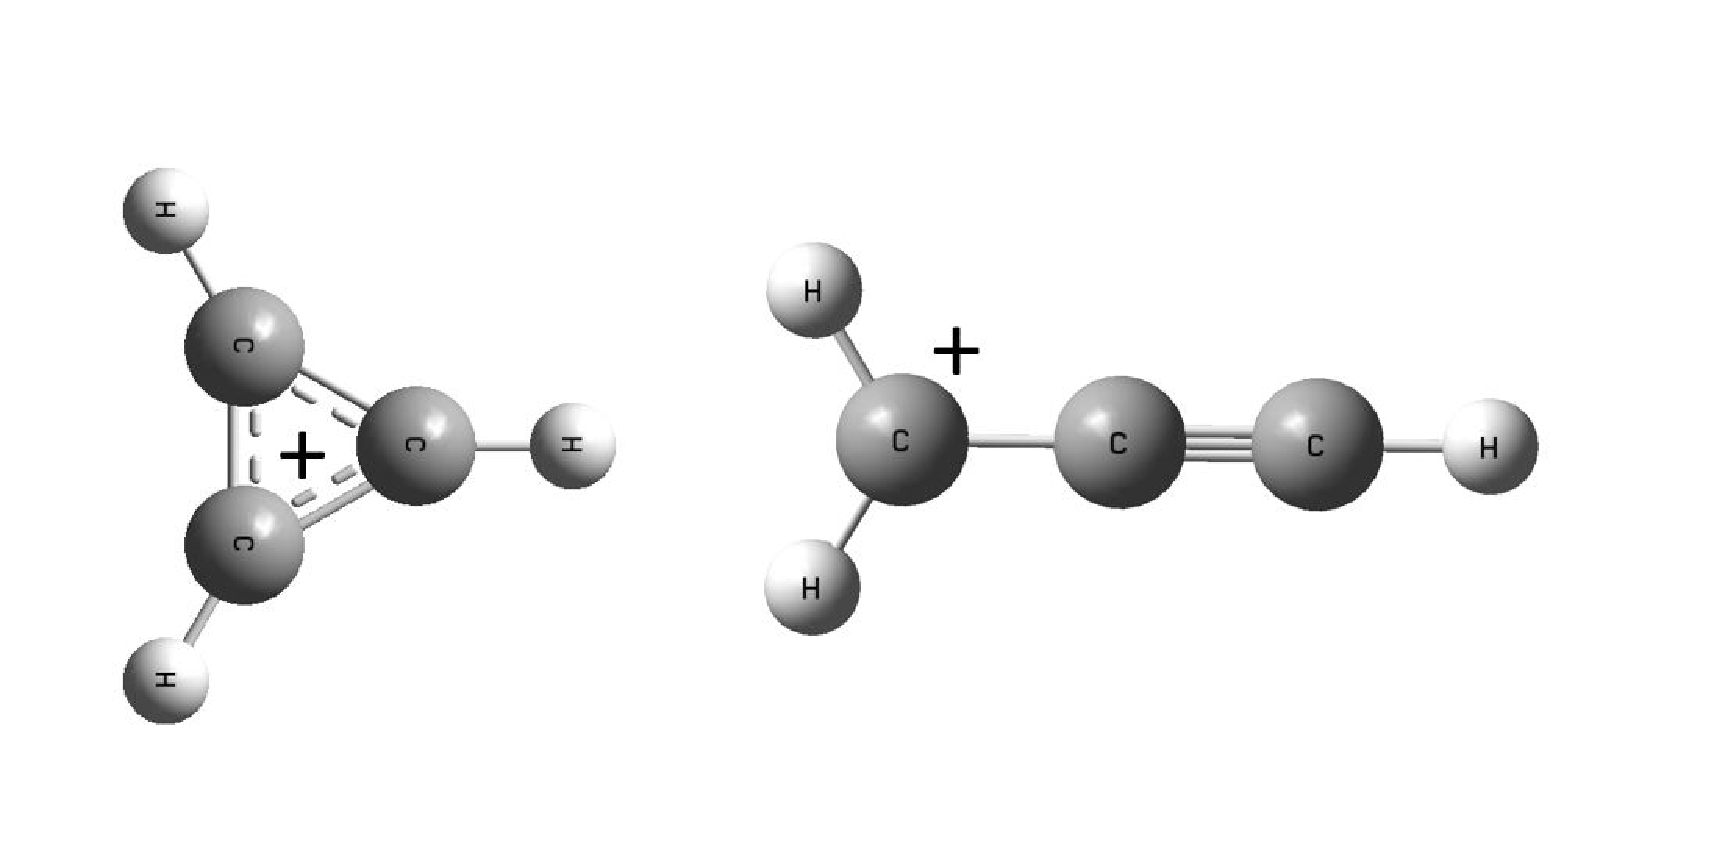
\includegraphics[scale=.4]{chapters/C3H3+ and C3D3+/figures/molecule.pdf}
		\caption{Molecular structures of \cyc (left) and \lin (right) isomers.}
	\label{FIG:C3H3+:molecule}
\end{figure}

\section{Methods}

\subsection{Experimental details}
\vspace{0.5cm}

\begin{figure}

	\centering
		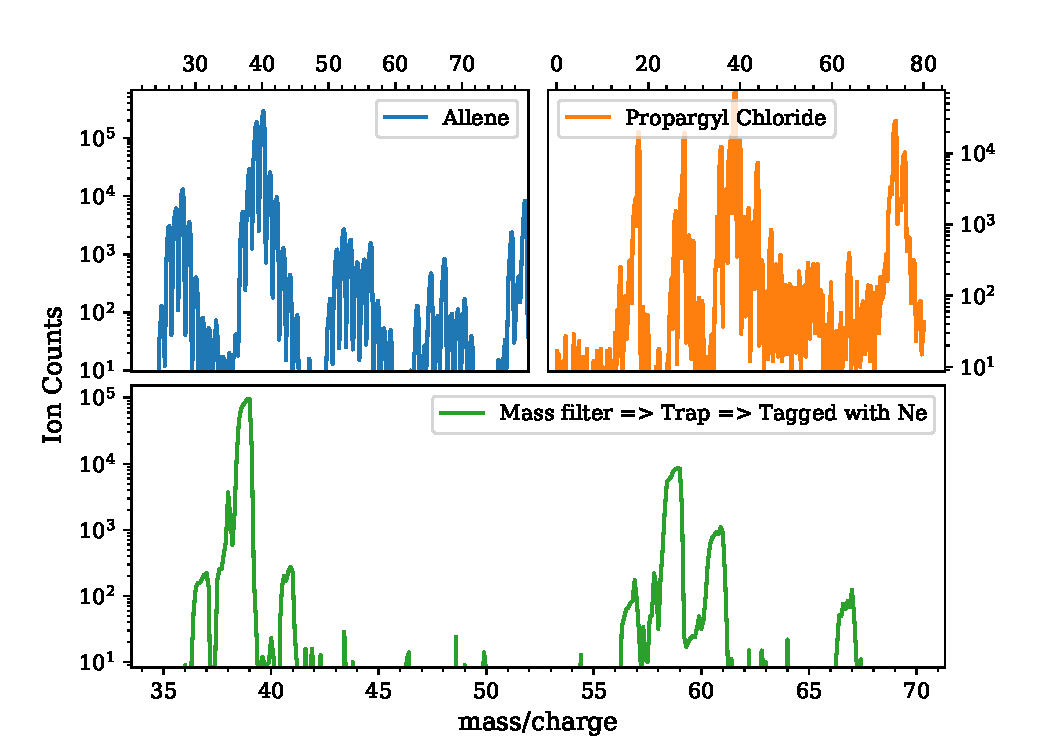
\includegraphics[scale=.7]{chapters/C3H3+ and C3D3+/figures/masspec.pdf}
		
	\caption{Mass spectra of ions produced from electron impact ionization (20~eV) of allene (left, in storage EI source) and propargyl chloride (right, in direct EI source) precursors (upper panel), and of mass filtered \iso (m = 39~u) together with tagged Ne-\iso (m = 59~u) species produced in the cryogenic ion trap (lower panel).}
	
	\label{FIG:C3H3+:masspec}
\end{figure}

The vibrational spectra of the \iso isomers and isotopologues were recorded using the FELion cryogenic 22-pole ion trap instrument located at the Free Electron Lasers for Infrared eXperiments (FELIX) Laboratory (see Section \ref{subsec:ir:radiation-source:FELIX}). A detailed account of the FELion instrument is provided in Section \ref{sec:felion} and the infrared-predissociation (IRPD) of in-situ rare gas tagged cold molecular ions in Section \ref{subsec:action:methods:vibrational:IRPD}. Here we only give a brief account of details specific to the \iso system. \\

Isomeric variants of \iso (m=39~u) were produced by electron impact ionization (electron energy $11-70$~eV) from neutral allene (C$_3$H$_4$, abcr GmbH, 96~\%)  and propargyl chloride (HC$_3$H$_2$Cl, Sigma Aldrich, 98~\%). Fully deuterated [C$_3$D$_3$]$^+$ was produced from deuterated allene (C$_3$D$_4$, Qmx Laboratories, 98~\%). The precursor gases were admitted either pure or diluted with He at a ratio of 1:3 to the ion source chamber at a pressure of $\sim 10^{-5}$~mbar. For most experiments, a simple electron-impact (EI) source was used, and additional measurements were done with a Gerlich-type storage ion source (SIS) \cite{Gerlich1992}, where primary ions produced by EI are accumulated for the duration of an experimental cycle (of the order of seconds), thereby allowing further reactions with the present neutral gas (see Figure \ref{FIG:C3H3+:masspec}).\\

For spectroscopic experiments a few 10~ms long pulse of ions is extracted from the respective source and filtered for the mass of interest, m=39~u in the case of \iso and m=42~u for [C$_3$D$_3$]$^+$, by a quadrupole mass selector before entering the 22-pole ion trap which is held at a fixed temperature in the range 6.1-7~K for experiments using Ne and 11~K for those using H$_2$ as tagging gasses. Around 10-20~ms before the ions enter the trap, an intense 80-150~ms long Ne:He (or H$_2$:He) pulse (1:3 mixing ratio and number density of $\sim 10^{15}$~cm$^{-3}$) is admitted to the trap, leading to efficient collisional cooling of the ions to the ambient temperature. Under these conditions, several 10~\% of the primary ions form weakly bound complexes with Ne (or H$_2$), see Figure \ref{FIG:C3H3+:masspec}. The ions are stored for several seconds in the ion trap and are exposed to several laser pulses before extraction. An IRPD spectrum is recorded by mass-selecting and detecting the \ison-Ne(H$_2$) complex ions while tuning the laser frequency $\nu$. A relative depletion $D=1-\frac{N_{ON}(\nu)}{N_{OFF}}$ in the number of complex ions $N_{ON}(\nu)$ from the baseline value $N_{OFF}$ is observed upon resonant vibrational excitation. To account for varying laser pulse energy $P$, pulse number $n$, and for saturation effects, the signal is normalized prior to averaging using $I=\frac{- ln(N_{ON}(\nu)/N_{OFF})}{n\cdot P/(h\nu)}$, giving the intensity $I$ in units of relative cross-section per photon\footnote{This equation only holds for isomer-pure ionic samples. Saturation effects in isomeric mixtures are underestimated in this way, leading to varying intensity ratios in the presented spectra.}. After normalizing each measurement in this way, the final spectrum is then obtained by averaging using statistical binning with a typical bin size of 2.5~\wn. Line parameters such as band positions, intensities, and line widths (fwhm) are then obtained by fitting a multi-component Gaussian function to the experimental data, also providing statistical errors of the line parameters. \\

Additionally, we performed saturation depletion experiments (see section \ref{iso}) to quantify the isomeric ratio of the ionic mixture as described in detail previously \citep{JSB2018,jusko_felion_2019}. Here we used up to 46 laser pulses, resonant with an isomer-specific vibrational band position, to fully deplete (dissociate) just one isomer complex. The analysis of the depletion signal as a function of laser pulses, corrected for other loss-mechanisms, allows then to derive both the absorption-dissociation cross-section and the isomer abundance. \\

The vibrational IRPD spectra were recorded using the IR radiation of FEL-2 of the FELIX Laboratory in the frequency region 550-2400 cm$^{-1}$, also employing the 3rd harmonic mode of the FEL. The laser was operated at 5 or 10~Hz with macro pulse energies in the interaction region between 1.5-60~mJ, and for each datapoint $n=$3-66 pulses were admitted depending on the signal strength. The FEL was optimized for narrow bandwidth with a full width at half-maximum (fwhm) of $0.3-1$~\% of the center wavelength. Additional spectra were recorded in the C-H-stretching region between 2800-3400~\wn using a Laservision OPO/OPA system ($\sim 3$ \wn\ fwhm, 10 Hz, 5~ns pulses) with typical power of $\sim$ 7-10~mJ.\\



\subsection{Computational details} 
\vspace{0.5cm}

The \iso  system has previously been studied quantum-chemically on several occasions
and at various levels of theory  \citep{HTL2011,BOR2011,BO2011,Botschwina2011}.
In the present investigation of the hydrogenated and perdeuterated variants, quantum chemical calculations have been performed 
at the coupled-cluster singles and doubles (CCSD) level 
augmented by a perturbative treatment of triple excitations, CCSD(T) \cite{raghavachari_chemphyslett_157_479_1989}, 
together with atomic natural orbital (ANO0, ANO1, and ANO2) basis sets from
Alml\"of and Taylor \cite{almlof_JCP_86_4070_1987}. The ANO0, ANO1, and ANO2 basis sets consist of 13s8p6d4f2g to 3s2p1d, 4s3p2d1f, and 5s4p3d2f1fg contractions for C as well as 8s6p4d3f to 2s1p, 4s2p1d, and 4s3p2d1f contractions for H, respectively. Equilibrium geometries have been calculated using analytic gradient techniques
\cite{watts_chemphyslett_200_1-2_1_1992}, while
harmonic frequencies have been computed using analytic second-derivative techniques
\cite{gauss_chemphyslett_276_70_1997,stanton_IntRevPhysChem_19_61_2000}.
For anharmonic calculations, second-order vibrational perturbation theory (VPT2) \cite{mills_alphas}   
has been employed and additional numerical differentiation of analytic second derivatives has been applied 
to obtain the third and fourth derivatives required for the application of VPT2  \cite{stanton_IntRevPhysChem_19_61_2000,stanton_JCP_108_7190_1998}.
The frozen core approximation has been used throughout.
All calculations (including those employing VPT2) have been carried out using the CFOUR program package \cite{cfour_JCP_2020,harding_parallel_2008}. \\

The CCSD(T) method in combination
with ANO basis sets has been shown previously to provide vibrational wavenumbers of high quality \cite{mccaslin_MolPhys_111_1492_2013,thorwirth_JMS_251_220_2008}.
In the present investigation, harmonic force fields were calculated at the
CCSD(T) /ANO2 level throughout. 
For the \cycD and \lin species, best estimates of the fundamental vibrational wavenumbers
were then calculated by applying anharmonic vibrational corrections 
calculated at the CCSD(T)/ANO1 level to the CCSD(T)/ANO2 harmonic wavenumbers.
Because of numerical problems in the CCSD(T)/ANO1 VPT2 calculation, for the 
\cyc and \linD species, anharmonic corrections were taken from corresponding CCSD(T) /ANO0 calculations. A comparison of the fundamental vibrational frequencies obtained in this fashion
using CCSD(T)/ANO1 and CCSD(T)/ANO0 for the \cycD and \lin species reveals that
the differences between the two levels are small, order of a few cm$^{-1}$ only.
From the anharmonic force field calculations we also find that in the \cycD species,
the $\nu_1$ mode is in resonance with the overtone of the $\nu_5$ mode
(using thresholds of $\Delta \omega = 50$\,cm$^{-1}$ and $\Phi_{ijj}=80$\,cm$^{-1}$). 
The corresponding VPT2 frequencies were unperturbed by removing the term
involving the resonance denominators. VPT2 intensities are not unperturbed in the present version of CFOUR and are reported here as provided by the program.
To support the spectroscopic assignment of vibrational features other than the fundamentals,
overtone and combination modes were also derived from the CCSD(T)/ANO1 (\cycD and \linn) and
CCSD(T)/ANO0 (\cyc and \linDn) computations. 
A summary of the computational results is given as part of the electronic
supplementary material.\\


\section{Results and discussions}

\begin{figure}

	\centering
	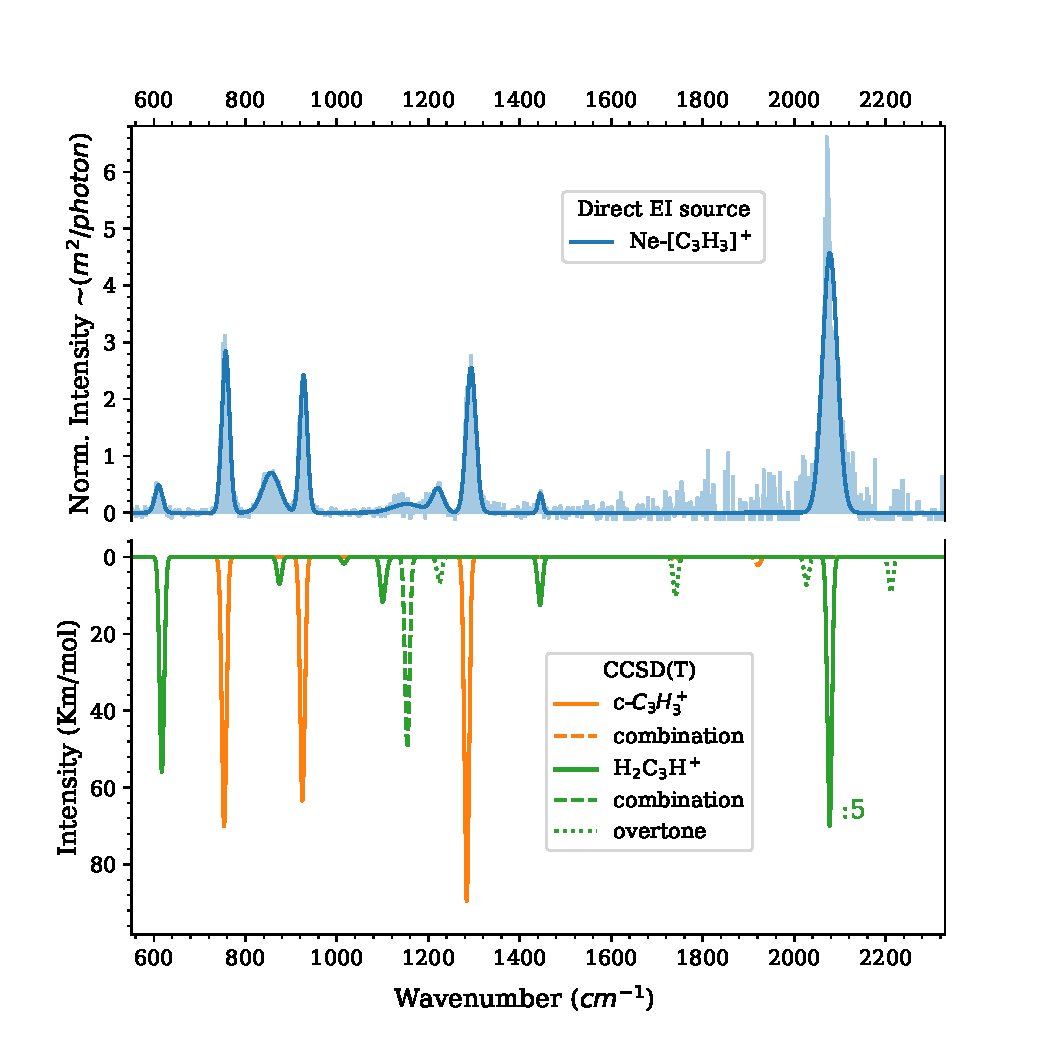
\includegraphics[width=1\textwidth]{chapters/C3H3+ and C3D3+/figures/felix_c3h3+.pdf}
	\caption{The experimental and fitted FELIX IRPD spectrum of Ne-\iso (upper panel) compared to computed frequencies (lower panel) at CCSD(T)/ANO2 combined with the anharmonic correction from CCSD(T)/ANO1 (\linn) and CCSD(T)/ANO0 (\cycn). Only fundamental  (solid line), combination (dashed line) and overtone (dotted line) infrared bands with intensity  $>\, \sim$1~km/mol were included. The theoretical spectrum was folded with a Gaussian corresponding to the FEL linewidth. Peaks marked with \textit{:n} indicate that the depicted peak intensity is scaled down by a factor n, for better visualization.}
	\label{FIG:felix}
\end{figure}

We measured experimental IRPD spectra of \iso isomers under various conditions such as using different ligands (Ne and H$_2$), ion sources (storage and direct EI sources, Figure \ref{FIG:compare_sources} ), and different precursors (propargyl chloride and allene) with ionization energy ranging from (14-70)~eV. The presence of both isomers with varying relative abundance in different conditions was observed and is discussed in detail in Section \ref{iso}. The IRPD vibrational band frequencies obtained from an average spectrum (Figure \ref{FIG:felix}, including data from the propargyl chloride and allene precursors produced in the direct EI source with varying electron impact energies) compared with computed and previous experimental frequencies of both isomers are summarised in Table \ref{tbl1}. The C-H stretching region was measured with the OPO/OPA system only for the allene precursor produced in the storage source, see Figure \ref{FIG:compare_ligands}. The vibrational band assignments based on various computational studies using coupled cluster methods will be discussed for the cyclic and linear isomer in detail in Sections \ref{cyclic} and \ref{linear}, respectively, and for the deuterated species in Section \ref{deut}. The influence of the tagging agent will be discussed in Section \ref{tag}, but was found to be negligible.  \\ 

\clearpage
% \begin{landscape}
\begin{ThreePartTable}
    \small
    \begin{TableNotes}\footnotesize
        \item [a] Frequencies (error in parenthesis). nc indicates not-covered and hyphen $-$ indicates not observed.\\
        \item [b] Measured with OPO/OPA system. The remaining bands are measured with the FELIX free electron laser.\\
        \item [c] Ref. \citep{GLY2012} - Velocity-map imaging photo-electron method.\\
        \item [d] Ref. \citep{Chin2018} -Direct IR absorption spectra of \lin in solid Ar matrix.\\
        \item [t] Tentative assignment.\\
        \item [*] Ref. \citep{RDS2010}.\\
     \end{TableNotes}
    \begin{longtable}{*{16}{c}}

        \caption{Summary of IRPD experimental vibrational band position of Ne-\iso compared to computed fundamental, overtone and combination band frequencies at the CCSD(T)/ANO2 level of theory combined with anharmonic corrections from CCSD(T)/ANO1 (for \lin) and CCSD(T)/ANO0 (for \cyc).}\label{tbl1}\\
        
        \toprule
        Mode & Ne-IRPD\tnote{a} & FWHM & Calc. [Int.]& Ar-IRPD \cite{RDS2010} & VMI-PE\tnote{c} & Ar-Matrix\tnote{d}\\
        & (this work)&\wn&\wn [Km/mol]& \wn& \wn& \wn\\
        
        \midrule
        \endfirsthead
        \\\\\hline \multicolumn{8}{c}{{\bfseries \tablename\ \thetable{} -- continued from previous page}} \\
        \toprule
        Mode & Ne-IRPD\tnote{a} & FWHM & Calc. [Int.]& Ar-IRPD \cite{RDS2010} & VMI-PE\tnote{c} & Ar-Matrix\tnote{d}\\
        & (this work)&\wn&\wn [Km/mol]& \wn& \wn& \wn\\
    
        \toprule
        \endhead
    
        \midrule
        \insertTableNotes
        \\\\\hline \multicolumn{8}{c}{{\bfseries \tablename\ \thetable{} -- continued on next page}} \\ \hline
        \endfoot
        \bottomrule
        % \insertTableNotes
        \endlastfoot
        
    
        \cyc & & & \\\\
        $\nu_{1}(a^{'}_1)$   &    -           & -  & 3179 [0]  & -    \\
        $\nu_{2}(a^{'}_1)$   &    -           & -  & 1610 [0]  & -    \\
        $\nu_{3}(a^{'}_2)$   &    -           & -  & 1024 [0]  & -    \\
        $\nu_{4}(e^{'})$     & 3133(1)\tnote{b}  & 14 & 3127 [189] & 3182 \\
        $\nu_{5}(e^{'})$     & 1293(1)        & 25 & 1284 [88] & 1293 \\
        $\nu_{6}(e^{'})$     & 927(1)         & 19 & 925 [60]  & nc   \\
        $\nu_{7}(a^{''}_2)$  & 757(1)         & 20 & 754 [70]  & nc   \\
        $\nu_{8}(e^{''})$    &    -           & -  & 1000 [0]  & -    \\
        \\
        $\nu_{7}$+$\nu_{8}(e^{'})$ & - & - & 1739 [1]  &      &          &          \\
        $\nu_{3}$+$\nu_{6}(e^{'})$ & - & - & 1921 [2]  &      &          &          \\\\
        \midrule
        
        \lin &&&&& \\\\
        
        %&----------- fundamental ------------\\
        $\nu_{1}(a_1)$                & -           & -  & 3230 [102] & 3238 &          & 3195.3   \\
        $\nu_{2}(a_1)$                & 3003(1)\tnote{b, t} & 9  & 2997 [26]  & 3004 &          & 3000.6   \\
        $\nu_{3}(a_1)$                & 2078(1)     & 32 & 2078 [346] & 2077 & 2086(15) & 2075.2   \\
        $\nu_{4}(a_1)$                & 1445(1)     & 12 & 1444 [12]  & 1445 &          & 1433.2   \\
              
        $\nu_{5}(a_1)$                & 1138(4)     & 31 & 1109 [2]   & 1222 & 1120(15) & 1140     \\
        $\nu_{6}(b_1)$                & 1138(4)     & 31 & 1100 [11]  & 1111 &          & 1105.2   \\
        $\nu_{7}(b_1)$                & 856(1)      & 44 & 875 [7]    & nc   & 858(15)  &          \\
        $\nu_{8}(b_1)$                & nc          & nc & 263 [26]   & nc   &          &          \\
        $\nu_{9}(b_2)$                &3041(1)\tnote{b, t}  & 9  & 3087 [37]  & 3093 &          & 3063.4   \\
        $\nu_{10}(b_2)$               & -           &  - & 1016 [2]   & -    &          &          \\
        $\nu_{11}(b_2)$               & 610(1)      & 12 & 618 [56]   & nc   &          & 606.8    \\
        $\nu_{12}(b_2)$               & nc          & nc & 299 [15]   & nc   &          &          \\\\
     
        %&----------- combination ------------\\
        $\nu_{3}$+$\nu_{5}(a_1)$      & -          &  - & 3168 [7]   &      &          &   \\
        $\nu_{3}$+$\nu_{10}(b_2)$     & -          &  - & 3086 [4]   &      &          &   \\
        $\nu_{4}$+$\nu_{10}(b_2)$     & -          &  - & 2444 [2]   &      &          &   \\
        $\nu_{7}$+$\nu_{8}(a_1)$      & 1138(4)    & 31 & 1154 [50]  &      &          &   \\\\
        
        %&----------- overtone ------------\\
        $2\nu_{4}(a_1)$               &  -          & -  & 2865 [1]   &      &          &   \\
        $2\nu_{5}(a_1)$               &  -          & -  & 2211 [9]   &      & 2247(15) &   \\
        $2\nu_{7}(a_1)$               &  -          & -  & 1741 [10]  &      & 1744(15) &   \\
        $2\nu_{10}(a_1)$              &             & 27 & 2027 [7]   &      &          &   \\
        $2\nu_{11}(a_1)$              & 1222(1)     & 27 & 1224 [7]   &      &          &   \\\\

    \end{longtable}
\end{ThreePartTable}
% \end{landscape}
% \clearpage

\subsection{Cyclic isomer}
\vspace{0.5cm}
\label{cyclic}
The planar \cyc isomer has $D_{3h}$ symmetry with an $A'_1$ vibronic ground state. All of the only four IR active fundamental bands ($\nu_4$, $\nu_5$, $\nu_6$ and $\nu_7$, with the former three being doubly-degenerate) of this energetically lowest-lying aromatic isomer are clearly observed (see Figure \ref{FIG:felix} and \ref{FIG:compare_ligands}, and Table \ref{tbl1}). The band at 3133 \wn\ is assigned to the $\nu_{4}$ asymmetric CH stretching mode, with good agreement to the computed value of 3127~\wn\ and to a previous Ne-IRPD experiment by Roth and Dopfer \cite{Roth2002}, who measured this band at 3130~\wnn. This vibration has also been reported in Ne-matrix at 3130 \wn\ \citep{Wyss2001}. Duncan and coworkers had originally  reported this band around 3182 \wn\ \citep{RDS2010}, but later revised their assignment \citep{Duncan2012}, in line with other experiments \citep{ZDL2014, Roth2002} (see Table \ref{tbl1}), including this work, and previous calculations \citep{BOR2011, HTL2011}. Based on their calculations, Botschwina et al. \citep{BOR2011} argued that the 3182~\wn\ band from Duncan's work could be the $\nu_3$+$\nu_5$ combination band of the linear isomeric form and not the $\nu_{4}$. The fact that we do not observe a band at 3182~\wn\ under conditions preferentially producing the cyclic isomer (see Section \ref{iso}), supports this assignment.
Somewhat puzzling is the appearance of two weak features at 3003 and 3041~\wn\, which are only present in the Ne-tagged spectrum in Figure \ref{FIG:compare_ligands}. No combination or overtone bands of the cyclic isomer are predicted at these frequencies. We tentatively assigned them to the $\nu_2$ and $\nu_9$ modes of the linear isomer. However, the much stronger $\nu_1$ band, observed at 3238~\wn\ in the Ne-IRPD spectrum of \citet{Botschwina2011}, is not detected.\\

The prominent feature $\nu_5(e')$ corresponding to the asymmetric CCC ring stretching is clearly identified at 1293~\wnn. This band was also reported at 1293 \wn\ with Ar-tagging \citep{RDS2010}. Whereas our computed anharmonic frequency at CCSD(T) level is lower by 11 \wnn, the comparison to CCSD(T) quartic force field calculations in combination with variational calculation (VCI 5MR) from \citet{HTL2011} shows good agreement (1296.2 \wnn). The in-plane CH scissoring (927 \wnn, $\nu_6(e')$) and symmetric CH out-of-plane wagging (757 \wnn, $\nu_7(a_2''$)) modes have been measured with an excellent agreement to the computed band positions (see Table \ref{tbl1}), and gas-phase data of these two bands are reported here for the first time. Previously, they were measured by Craig et al. \citep{Craig1986} in various different polycrystalline salts of \cycn $X^{-}$ (with X=SbF$_5$) at  757 \wn\ ($\nu_7$) and 925 \wn\ ($\nu_6$) which agree well with our measurements.\\

\subsection{Linear isomer}
\label{linear}
\vspace{0.5cm}
The linear propargyl isomer with $C_{2v}$ symmetry and an $A_1$ vibronic ground state has 12 fundamental bands, which are all IR active. Previous measurements on the gas-phase \lin isomer include Ar-IRPD spectra (at frequencies above the Ar binding energy ($\sim$ 1000~ \wn)) \citep{RDS2010} and combined vacuum ultraviolet (VUV) laser - velocity-map imaging photoelectron (VMI-PE) spectra obtained only for the $\nu_3$, $\nu_5$ and $\nu_7$ modes \citep{GLY2012}. Here we report and discuss the spectral characterization of the \lin isomer measured in a wide range from 550-3400 \wn. \\

The most prominent $\nu_3(a_1)$ CC triple bond stretching mode at 2078 \wn\ is clearly seen with an excellent agreement to the computed value of the bare ion (2078~\wnn) and the experimental value (2077~\wnn) obtained with Ar-tagging IRPD \citep{RDS2010}. Similarly, the weak band at 1445~\wn\ is assigned to the $\nu_4$ CH$_2$ scissoring vibration. The broad mode identified at 1222~\wn\ can be assigned to $2\nu_{11} (a_1)$ supported by a computed value of the overtone at 1224~\wn\ with substantial intensity larger than other overtone and combination bands in that region. This band was originally assigned to the $\nu_5$ band by Ricks et al. \citep{RDS2010}.  The similarly broad band at 1138 \wn\ with larger uncertainty of 3-4~\wn\ and FWHM of 31~\wn\ is consequently assigned here to a blend of $\nu_5$, $\nu_6$, and $\nu_7+\nu_8$ (intensity of this combination mode might be over-estimated in the calculation, ~50 km/mol, see Figure \ref{FIG:felix}), which our anharmonic CCSD(T) calculations predict at 1109, 1100, and 1154 \wnn, respectively. We should, however, note here that our calculated $\nu_5$ and $\nu_6$ band position are not consistent with the earlier coupled cluster calculations from Botschwina and co-workers \citep{Botschwina2011, BOR2011} and Huang et al. \citep{HTL2011} (see Table \ref{tab:tbl_compare_calc}), who predicted these bands at 1123~\wn\ and 1100~\wnn, respectively, for Ne-tagged \lin and around 1130~\wn\ and 1058~\wn\ (depending on the level of theory), respectively, for the bare ion. The discrepancy for the $\nu_5$ band is likely due to varying theoretical treatment of a Fermi resonance with the $\nu_7+\nu_8$ combination band, which might be further influenced by the (small) perturbation of the Ne-tag. Ricks et al. \citep{RDS2010} observed a doublet feature centered at 1111~\wn\ with Ar as tagging agent, and assigned it to the partly resolved P- and R-branch of the perpendicular $\nu_6$ band.  The $\nu_7$ CCH out-of-plane bending and $\nu_{11}$ CCH in-plane bending bands clearly appear at 856 and 610~cm$^{-1}$, respectively. However, the former band is extremely broad, as is the equivalent band in the fully deuterated species, and was difficult to distinguish from baseline fluctuations in the experiments. We assume a fast predissociation of the Ne-ion complex upon excitation of this mode, leading to life-time broadening. \\

\subsection{Ne-effect}
\vspace{0.5cm}
\begin{figure}
	\centering
	
		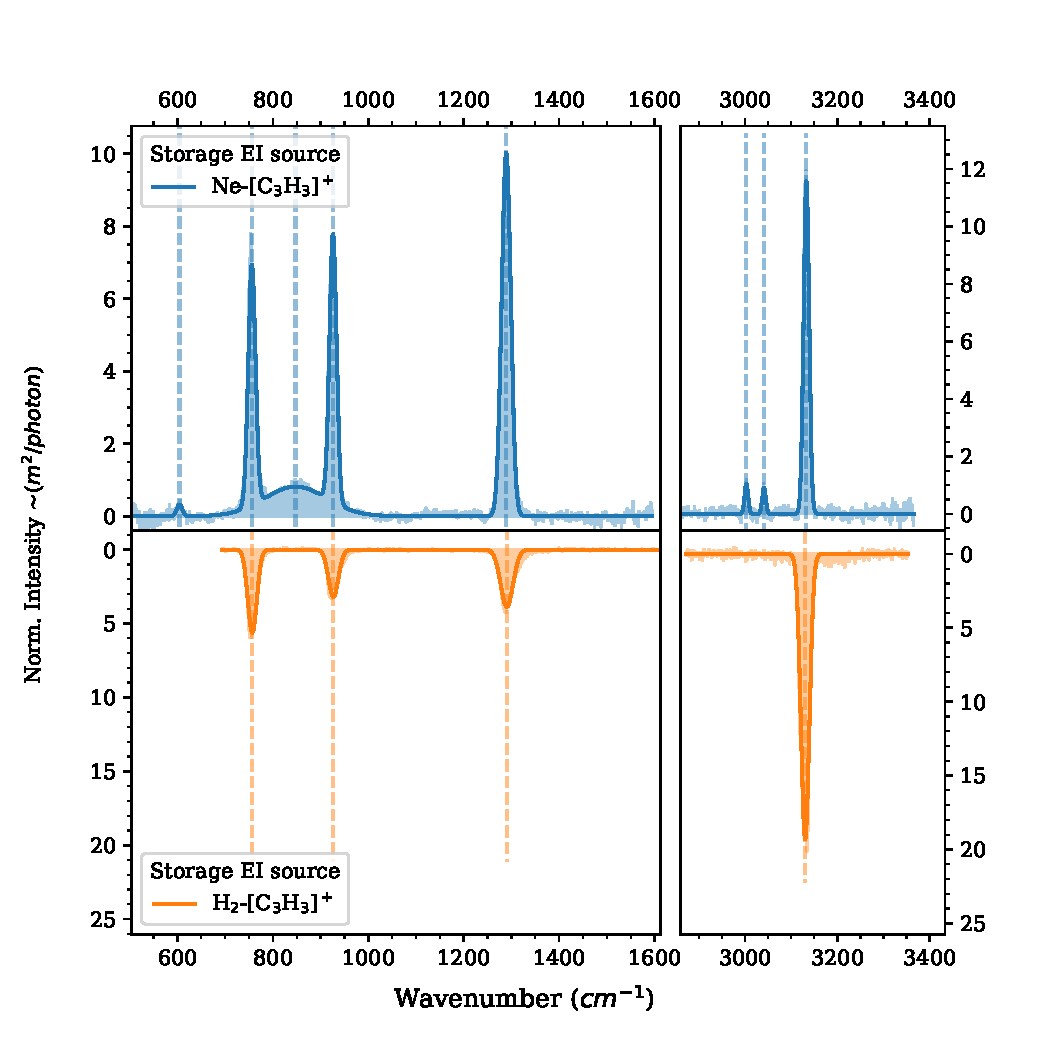
\includegraphics[scale=.7]{chapters/C3H3+ and C3D3+/figures/compare_ligands.pdf}
	\caption{Comparing Ne-\iso (upper panel) and H$_2$-\iso (lower panel) IRPD spectra produced from allene precursor in the storage ion source recorded with FELIX laser and OPO. }
	\label{FIG:compare_ligands}
\end{figure}


\begin{table}

    \caption{Comparing \lin Ne-IRPD band positions with available computational studies based on coupled cluster methods. All frequencies are in \wn\ units}\label{tag}
    \footnotesize
    \centering
    \begin{tabular}{lccccc}
    
        \hline \hline \\
        Mode& Ne-IRPD & \lin & Ne-\lin & Ar-\lin & \lin   \\
        & (this work)&(this work)$^a$& \multicolumn{2}{c}{\citet{Botschwina2011}$^b$} & \citet{HTL2011}$^c$\\
        \hline\\
        $\nu_{1}(a_1)$  &      & 3230 & 3237(+1) & 3241(+5) & 3239.0 \\
        $\nu_{2}(a_1)$  & 3003$^t$ & 2997 & 2992(+2) & 2996(+6) & 2998.7 \\
        $\nu_{3}(a_1)$  & 2078 & 2078 & 2080(0)  & 2081(+1) & 2082.2 \\
        $\nu_{4}(a_1)$  & 1445 & 1444 & 1446(0)  & 1446(0)  & 1434.4 \\
        $\nu_{5}(a_1)$  & 1138 & 1109 & 1123(0)  & 1119(-4) & 1131.8 \\
        $\nu_{6}(b_1)$  &      & 1100 & 1100(+1) & 1097(-2) & 1058.1 \\
        $\nu_{7}(b_1)$  & 856  & 875  & 873(+1)  & 867(-5)  & 861.9  \\
        $\nu_{8}(b_1)$  &      & 263  & 264(0)   & 281(+17) & 251.7  \\
        $\nu_{9}(b_2)$  & 3041$^t$ & 3087 & 3082(+2) & 3086(+6) & 3071.0 \\
        $\nu_{10}(b_2)$ &      & 1016 & 1017(0)  & 1017(0)  & 1000.6 \\
        $\nu_{11}(b_2)$ & 610  & 618  & 615(0)   & 618(+3)  & 607.7  \\
        $\nu_{12}(b_2)$ &      & 299  & 301(+3)  & 302(+4)  & 294.8  \\
        
        \hline\hline\\
    \end{tabular}\\
    $^a$ Computed at CCSD(T)/ANO2 combined with anharmonic correction from ANO1\\
    $^b$ $C_s$ min1 structure computed at CCSD(T)-F12/VTZ-F12. Harmonic shift arising from complex formation is given in parentheses.\\
    $^c$ Computed at CCSD(T) QFF with VCI 5MR method. Note that the symmetry labelling of b1 of \citep{HTL2011} is b2 in this paper.\\
    $^t$ Tenative assignment.
    \label{tab:tbl_compare_calc}
\end{table}

We analyzed the effect of Ne complexation on the bare ions' vibrational spectra by comparing them to the computed anharmonic frequencies from various coupled cluster methods of both ligand tagged and untagged species. Botschwina and co-workers \citep{Botschwina2011} had carried out very detailed computational studies on the weak interactions in the ion-ligand complexes of \iso by analyzing the potential energy profile of the complexes while migrating the ligand around the ion-molecule. They have found two $C_s$ and one $C_{2v}$ (highest energy) structures for Ne-\cyc and three $C_s$ minima for Ne-\lin complex ion. They found negligible shifts of order $<3$~\wn\ for the vibrational band positions for both \iso isomers and all ligand-ion isomers. A detailed comparison of ligand-induced band shifts in the spectrum of the \lin isomer is provided in Table \ref{tab:tbl_compare_calc}, where we report only values for the lowest energy $C_s$ structure from \citet{Botschwina2011}. The prominent features $\nu_3$ and $\nu_4$ appear to have no perturbation within 1~\wn\ uncertainty and this is supported by both our Ne-IRPD experiment and calculations on Ne-\linn. The larger discrepancy in the $\nu_7$ band could be reasonably explained by other effects as discussed in section \ref{linear} and \ref{deut}. The four IR active fundamental band of the cyclic isomer of both \iso (except $\nu_5$, see section \ref{cyclic}) and \isoD (section \ref{deut}) also show excellent agreement with the computed fundamental band positions. \\

We can therefore take the IRPD spectra of the Ne-tagged species as an excellent proxy for those of the bare ion, with predicted vibrational shifts much smaller than those for the corresponding Ar-tagged species. Surprisingly, even the use of H$_2$, which has much higher polarizability than Ne (4.5~a.u.  \citep{MH2018} {\textit{vs.}} 2.66~a.u. \citep{SN2018}, respectively) as the tagging agent does not lead to significant shifts, as the comparison in Figure \ref{FIG:compare_ligands} shows, taken under conditions favoring the formation of the \cyc isomer. The predicted small ($\sim 1$~\wnn) splitting of the degenerate e' modes ($\nu_4$, $\nu_5$, and $\nu_6$) of \cyc caused by symmetry-breaking due to the ligand could not be resolved with the given laser linewidth in these experiments. \\



\subsection{Deuterated species}
\label{deut}
\vspace{0.5cm}

Figure \ref{FIG:felix_c3d3+} shows the IRPD spectra of Ne-tagged \isoDn, produced in the direct EI source from fully deuterated allene (C$_3$D$_4$) as a precursor. We covered the range 400-2600~\wnn; using the FEL in its $3^{rd}$ harmonic mode in the range (1800-2600 \wnn), where the substantially shifted C-D stretching bands are expected. The first comprehensive spectral characterization of \cycD was reported by \citet{Craig1986} using poly-crystalline salts. For the linear form \linDn, the C$\equiv$C stretching $\nu_3$ band in Ne-matrix \citep{Wyss2001} and the $\nu_1$-$\nu_6$, $\nu_9$ bands from a recent study of direct absorption of IR bands using isolated solid Ar matrix techniques \citep{Chin2018} were previously reported. However, to the best of our knowledge, there are no reports available on gas-phase data. Hence, here we report the first gas-phase data for \isoD isomers.\\ 

\begin{figure}
	\centering
		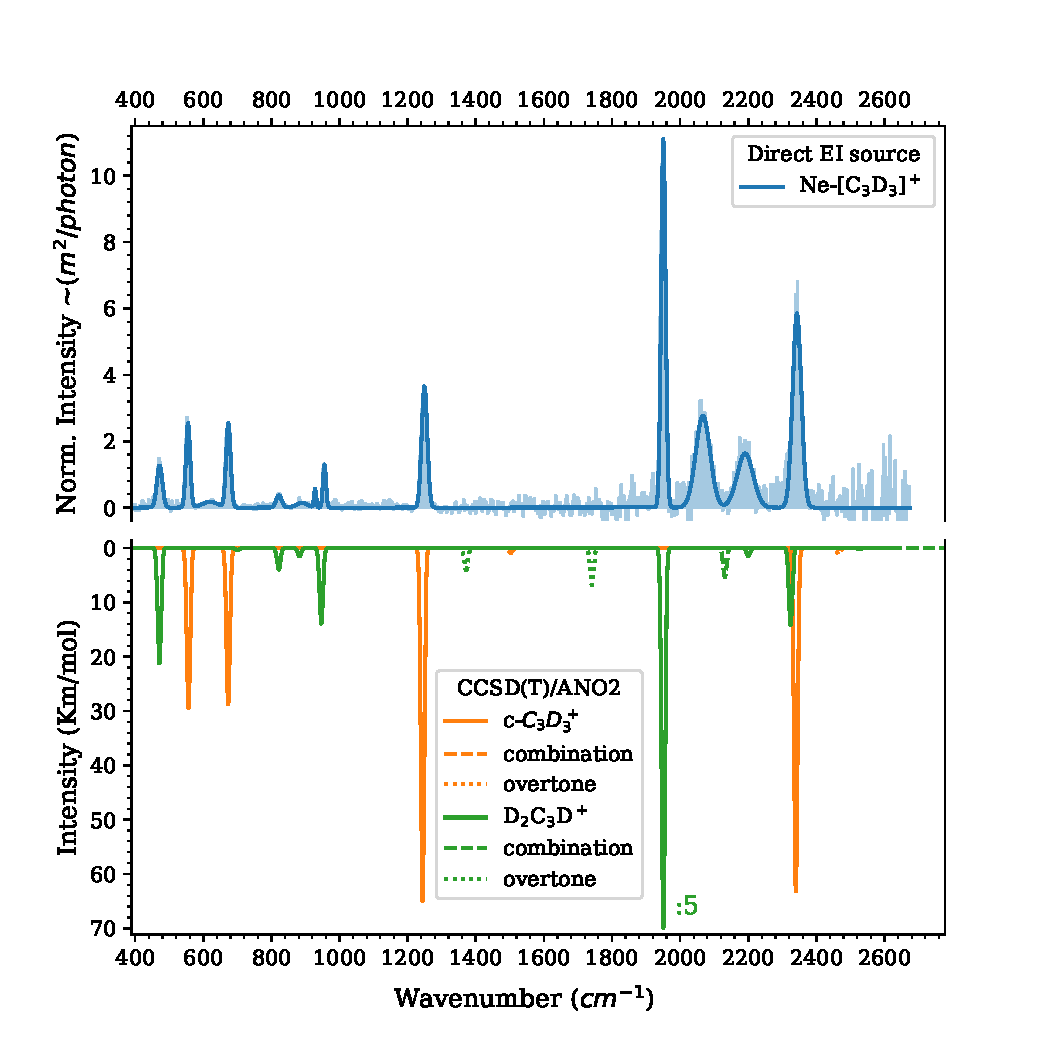
\includegraphics[scale=.7]{chapters/C3H3+ and C3D3+/figures/felix_c3d3+.pdf}
	\caption{The experimental and fitted FELIX IRPD spectrum of Ne-\isoD (upper panel) compared to computed frequencies (lower panel) at CCSD(T)/ANO2 combined with the anharmonic correction from CCSD(T)/ANO1 (\cycDn) and CCSD(T)/ANO0 (\linDn). Only fundamental (solid line) combination (dashed line) and overtone (dotted line) infrared bands with intensity $>\, \sim$1~km/mol were included. The theoretical spectrum was folded with a Gaussian corresponding to the FEL linewidth. Peaks marked with \textit{:n} indicate that the depicted peak intensity is scaled down by a factor n, for better visualization.}
	\label{FIG:felix_c3d3+}
\end{figure}

\clearpage
\begin{landscape}
\begin{ThreePartTable}
    \begin{TableNotes}\footnotesize
        \item [a] Frequencies (error in parenthesis). nc indicates not-covered and hyphen $-$ indicates not observed. $\oplus$ indicates out-of-plane\\
        \item [b] Blended with the $\nu_4$ band of \cycD at 2343~\wn. \\
        \item [c] \citet{Craig1986}, Infrared spectra with polycrystalline salts (\iso BF$_4^-$). \\
        \item [d] \citet{Wyss2001}, Infrared spectra in Neon matrix. \\
        \item [e] \citet{Breslow1970}, Infrared spectra from salts of deuterated cyclopropenyl cation. \\
        \item [f] \citet{Chin2018}, Infrared spectra of \lin in solid Ar matrix\\
     \end{TableNotes}
    \begin{longtable}{*{16}{c}}

        \caption{Summary of IRPD experimental vibrational band position of Ne-\isoD compared to computed fundamental, overtone and combination band frequencies at the CCSD(T)/ANO2 level of theory combined with anharmonic corrections from CCSD(T)/ANO1 (for \cycD) and CCSD(T)/ANO0 (for \linD).}\label{tab:c3d3+}\\
        
        \toprule
        Mode & Assignment & Ne-IRPD         & FWHM & Calc. [Int.] & Prev. Exp.  \\
             &            &(this work) \tnote{a} & \wn  & \wn [Km/mol] & \wn          \\
        
        \midrule
        \endfirsthead
    
        \\\\\hline \multicolumn{8}{c}{{\bfseries \tablename\ \thetable{} -- continued from previous page}} \\
        \toprule
        Mode & Assignment & Ne-IRPD         & FWHM & Calc. [Int.] & Prev. Exp.  \\
             &            &(this work) \tnote{a} & \wn  & \wn [Km/mol] & \wn          \\

        \toprule
        \endhead
    
        \midrule
        \insertTableNotes

        \\\\\hline \multicolumn{8}{c}{{\bfseries \tablename\ \thetable{} -- continued on next page}} \\ \hline
        \endfoot
        \bottomrule
        % \insertTableNotes
        \endlastfoot
    
        \hline
        \hline \\
        
             
        \hline\\
        \cycD &&&& \\\\
        %&----------- fundamental ------------\\
        $\nu_{1}(a^{'}_1)$ & sym. CD str.              &    -    &  -  & 2474 [0]  \\
        $\nu_{2}(a^{'}_1)$ & sym. CCC str.             &    -    &  -  & 1478 [0]  \\
        $\nu_{3}(a^{'}_2)$ & in-plane internal torsion &    -    &  -  & 838  [0]   \\
        $\nu_{4}(e^{'})$   & asym. CD str              & 2343(1) & 30 & 2340 [64] & 2348\tnote{c}, 2344.1(1.0)\tnote{d}, 2327\tnote{e}  \\ 
        $\nu_{5}(e^{'})$   & asym. CCC ring str.       & 1249(1) & 25 & 1244 [65] & 1250\tnote{c}, 1239\tnote{e} \\
        $\nu_{6}(e^{'})$   & in-plane CD scissoring    & 674(1)  & 19 & 673  [28] & 670\tnote{c}, 665\tnote{e} \\
        $\nu_{7}(a^{''}_2)$& sym. CD bending $\oplus$  & 556(1)  & 15 & 556  [27] & 542 \tnote{c}, 542\tnote{e} \\
        $\nu_{8}(e^{''})$  & asym. CD bending $\oplus$ &    -    &  -  & 817  [0]   \\\\
        
        
        %&----------- combination ------------\\
        $\nu_3$+$\nu_5(e^{'})$ &   & 2067(1) & 49 & 2061[0.02]  \\\\
        %$\nu_3$+$\nu_6(e^{'})$ &   &    -     &  -  & 1502[0.9]     \\\\
        
        %&----------- overtone ------------\\
        $2\nu_{5}(e^{'})$  & & - &- & 2466 [1]\\\\
        
        \midrule
        
        \linD &&&&& \\\\
        
        %&----------- fundamental ------------\\
        $\nu_{1}(a_1)$ & CD str.              & -       & -  & 2527 [0.2] & 2487.3\tnote{f} \\
        $\nu_{2}(a_1)$ & CD$_2$ sym str.      & 2193(1) & 55 & 2200 [1.5]  & 2201.0\tnote{f}\\
        $\nu_{3}(a_1)$ & C$\equiv$C str.      & 1951(1) & 32 & 1951[350] & 1955.2(1.0)\tnote{d}, 1942.1\tnote{f}\\
        $\nu_{4}(a_1)$ & CD$_2$ scissoring    & -       & -  & 1201 [0.09] & 1191.7\tnote{f}\\
        $\nu_{5}(a_1)$ & C-C str.             & 956(1)  & 10 & 946 [14] & 938.7\tnote{f}  \\
        %\textcolor{red}{$\nu_8$+$\nu_{10}$ (a$_2$)} &&&& 1056 [0] \\
        $\nu_{6}(b_1)$ & CD$_2$ wag $\oplus$    & 883(3)         & 16 & 882 [1.5] & 891.3\tnote{f}      \\
        $\nu_{7}(b_1)$ & CCD bend $\oplus$      & 619(5)         & 54 & 700 [0.3]                   \\
        $\nu_{8}(b_1)$ & CCC bend $\oplus$      & nc             & nc & 233 [16]                    \\
        $\nu_{9}(b_2)$ & CD$_2$ asym str.       & not resol.\tnote{b} &    & 2324 [14] & 2301.9\tnote{f}     \\
        $\nu_{10}(b_2)$& CD$_2$ wag $\oplus$    & 822(2)         & 20 & 822 [4]                   \\
        $\nu_{11}(b_2)$& CCD bend in-plane      & 472(1)         & 19 & 471 [21]                    \\
        $\nu_{12}(b_2)$& CCC bend in-plane      & nc & nc        &     262 [10] &                   \\\\
        
        %&----------- combination ------------\\
        $\nu_{1}$+$\nu_{7}(b_1)$ & & -   &  -    & 3206 [1]\\
        $\nu_{4}$+$\nu_{5}(a_1)$ & & -   &  -    & 2132 [5]\\
        $\nu_{7}$+$\nu_{8}(a_1)$ & &928(1)& 7.7 & 914 [0.6]\\\\
        %&----------- overtone ------------\\
        $2\nu_{6}(a_1)$ &  & - & -& 1741 [7]\\
        $2\nu_{7}(a_1)$ &  & - & -& 1372 [5]\\\\
    \end{longtable}
\end{ThreePartTable}
\end{landscape}
\clearpage

We clearly identify the four IR active fundamental bands of the cyclic isomer ($\nu_4$, $\nu_5$, $\nu_6$ and $\nu_7$) with excellent agreement to computed fundamental band positions of the untagged species (see Table \ref{tab:c3d3+}). This again demonstrates that the perturbation due to Ne attachment is very small. We also notice an additional feature, with a larger FWHM of 49 \wn, at 2067~\wnn. This band can be assigned to the (weak) predicted combination band $\nu_3$+$\nu_5$ at 2061~\wn.
For the \linD isomer, the $\nu_2$, $\nu_3$, $\nu_5$, $\nu_6$, $\nu_7$, $\nu_{10}$, and $\nu_{11}$ vibrational modes are clearly identified. The most prominent feature is the C$\equiv$C stretching ($\nu_3$) band observed at 1951~\wn. This band was reported at 1955.2~\wn\ in Neon matrix \citep{Wyss2001}. Most bands are in good agreement with theory (see Table \ref{tab:c3d3+}). The $\nu_7$ is assigned to the broad feature centered at 619~\wn\ and shows a large deviation to the calculated band position. Interestingly, a similar situation was observed for the corresponding band in the undeuterated species (see Table \ref{tbl1}). 
%We assign the band at 956~\wn to the $\nu_5$ C-C stretching mode based on the previous Ar-matrix data \citep{Chin2018}, even though we observe a large deviation to the calculated band position of 1052~\wn.
An additional band observed at 928~\wn\ is assigned to the $\nu_7+\nu_8$ combination band predicted at 914~\wnn.\\


\subsection{Isomer quantification}
\label{iso}
\vspace{0.5cm}
\begin{figure}
	\centering
		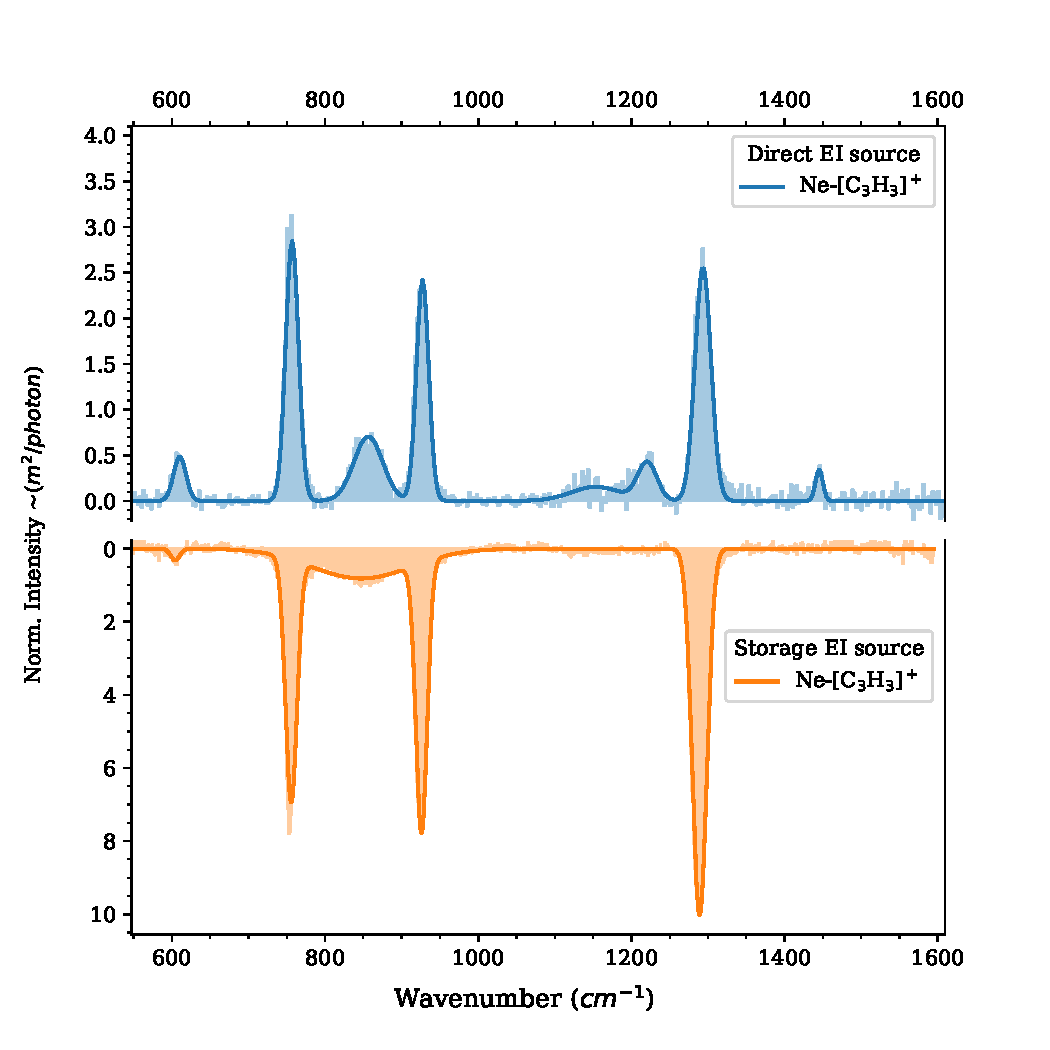
\includegraphics[scale=.7]{chapters/C3H3+ and C3D3+/figures/compare_ion_sources.pdf}
    	\caption{Isomer variation depending on ion production conditions. Upper panel: Experimental IRPD spectrum of Ne-\iso produced from propargyl chloride in the EI source. Lower panel: Same as above but using an allene precursor and the storage ion source.}
    	\label{FIG:compare_sources}
    	
\end{figure}

\begin{figure}
	
	\centering
		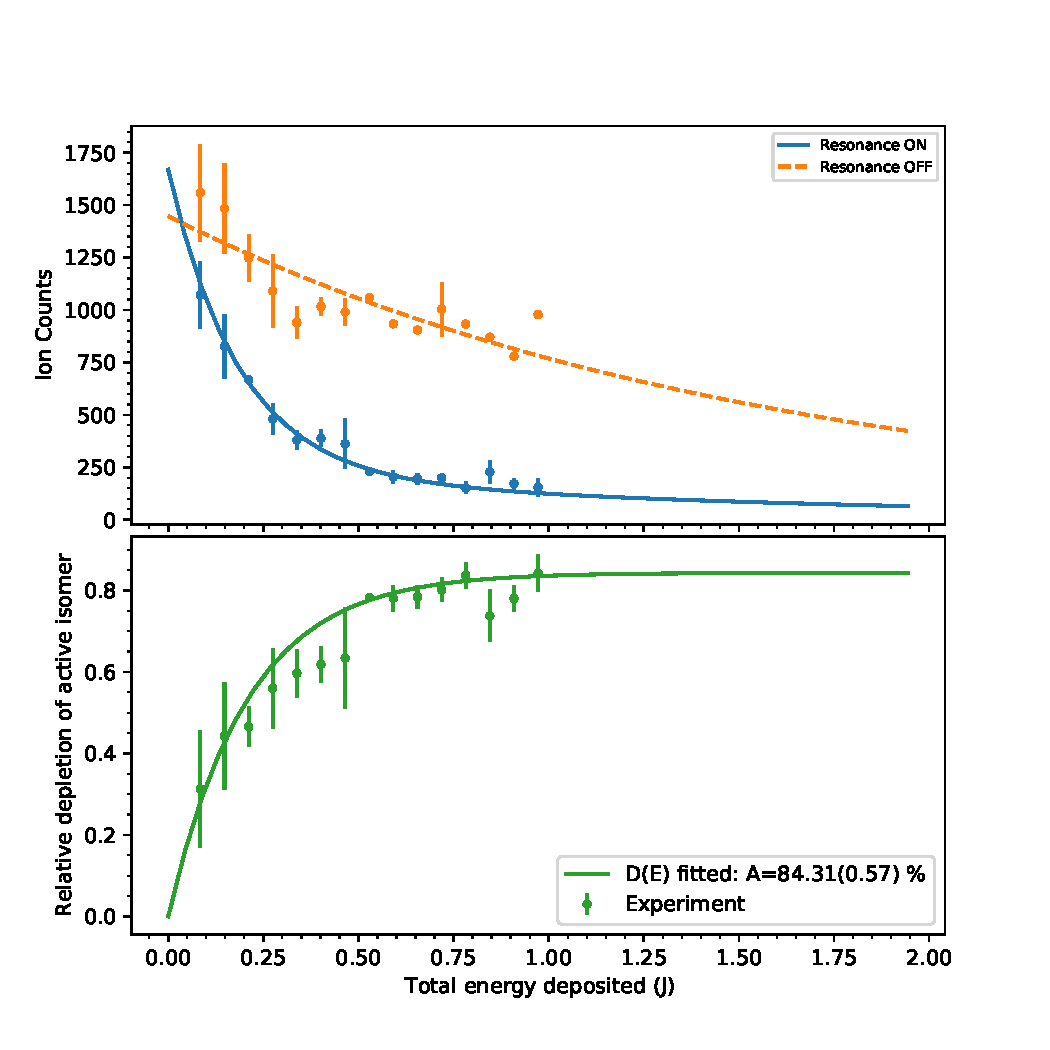
\includegraphics[scale=.7]{chapters/C3H3+ and C3D3+/figures/scan2.pdf}
	\caption{Saturation depletion measurements on the $\nu_5$ band of \cyc, produced from propargyl chloride in the direct EI ion source with ~16.5 eV electrons. Top: On-resonance (blue, at 1293~\wnn, $\nu_5$) and off-resonance (orange, at 1150~\wnn) depletion measurement. Bottom: Relative depletion $D(E)$ as a function of deposited energy $E$, showing saturation at $A=84$\%. }
	\label{FIG:depletion1}
	
\end{figure}

One of the goals of this study was to find ion production methods that preferentially form one of the two \iso isomers, in order to perform subsequent ion-molecule reaction kinetic studies starting with an isomer-pure ionic sample. For this purpose, we used two different neutral precursors, allene and propargyl-chloride, two different ion sources, and a range of electron impact energies.\\

As was described previously \citep{jusko_felion_2019,JSB2018}, it is possible to quantify the percentage of a specific isomer in an isomeric mixture by a saturation depletion method. For this the cluster is resonantly excited at a frequency where only one of the two isomers is active, i.e. absorbs a photon. By increasing the trapping time, thereby increasing the total energy ($E=n\cdot P$) deposited, only the active isomer cluster is depleted until it saturates, and the number of clusters is recorded as a function of deposited energy ($N_{ON}(E)$). To account for additional loss mechanisms from the trap, a second measurement is done with the laser tuned to an off-resonance position, resulting in $N_{OFF}(E)$. From this we can quantify the relative depletion of the particular isomer $D(E)=1-\frac{N_{ON}(E)}{N_{OFF}(E)}$. Assuming an  exponential decay of the clusters with rate coefficients $K_{ON}$ and $K_{OFF}$, respectively, we can write:
\begin{align*}
 N_{OFF}(E) &=  N \cdot e^{-K_{OFF}\cdot E}\\
%\label{eqn:Noff}
 N_{ON}(E) &=  N_a \cdot e^{-(K_{OFF}+K_{ON}) \cdot  E} + N_n \cdot  e^{-K_{OFF} \cdot E}\\
%\label{eqn:Non}
 D(E) &= 1-\frac{N_{ON}}{N_{OFF}} = A \cdot (1-e^{-K_{ON} \cdot E}),\\
\label{eqn:depletion}
\end{align*}
where  $N(=N_a + N_n)$, $N_a$ and $N_n$ are total cluster, active and non-active isomeric cluster counts respectively, and $A=\frac{N_a}{N_a + N_n}$ is the relative abundance of the active isomer. By fitting the experimental data to the corresponding exponentials, we can derive the respective rate coefficients, and, more importantly, the relative abundance of the targeted active isomer, $A$. Such an exemplary fit is shown in Figure \ref{FIG:depletion1}. We should note that this method assumes an equal probability for forming Ne complexes for different isomers. This can be safely assumed, since the binding energies for both Ne-\iso isomers was calculated to be very similar \citep{Botschwina2011}.\\

Although for the \iso ions the cyclic \cyc is substantially lower in energy than the linear \lin form  (28 ~kcal/mol,  \citep{HTL2011}), both isomers were regularly observed in various experiments \citep{RDS2010, Wyss2001, DRM2002}, including this work. Presumably, due to the high isomerization barrier between the two isomers (50~kcal/mol),  both isomers can be formed in the dissociative ionization of the used precursor gases. Theoretical studies have for example shown that the allene and propyne cations, with a linear carbon backbone, can undergo isomerization and ring closure before hydrogen loss, forming dominantly the \cyc isomer upon dissociation \citep{FS1983,MB2008}. 
We indeed observed the cyclic isomer with an abundance of $\sim$81~\% (and the linear form with $\sim$19~\%) upon electron impact ionization of allene in a direct electron impact ionization source, independent of the chosen electron energy in the range $(14-70)$~eV, indicating a constant isomeric branching ratio once the dissociation threshold in the ionization process is reached (allene ionization potential 9.7~eV \citep{YWL1990}, \iso appearance energy 11.4~eV \citep{LOSSING1972}, below 14~eV we could not produce a high enough \iso ion number to perform spectroscopic measurements). When using an ion storage source instead, where the primary ions can undergo subsequent reactions with the neutral gas, we predominantly produced the cyclic form ($\sim$90-95~\%), indicative of the higher reactivity of the linear isomer \linn,  as discussed previously \citep{SLA1982,MMF1994}.\\

In order to increase the formation yield of the propargyl cation \linn, we also used propargyl chloride (ionization energy 10.68(3)~eV, \citep{TWB1975}) as a precursor for direct electron impact ionization. The reasoning here was that the chlorine is expected to be an efficient leaving group after ionization and that thus the propargyl structure is retained in the \iso ionic fragment, as has been proposed in photodissociation studies of the propargyl chloride ion \citep{KR1985}. A comparison between spectra taken under different conditions is given in Figure \ref{FIG:compare_sources}. However, the isomeric ratio shifted only marginally towards the linear isomer, reaching $\sim$22~\% at 60~eV electron impact energy, and being lower ($\sim$16~\%) than for allene ionization at 16.5~eV. \\


To elucidate the formation of the different isomers upon ionization of propargyl chloride, we performed calculations on the potential energy surface of the [ClC$_3$H$_3$]$^+$ system, which are detailed in the Supplementary Information (Figure \ref{fig:C3H3+:fig1}). Our results agree well with earlier calculations at a lower level of theory by \citet{WCK2000}. They indicate that the dissociation to \cyc and Cl via an isomerization to a cyclic form of [ClC$_3$H$_3$]$^+$ is thermodynamically favoured (with a maximum barrier of 53.4~kJ/mol, i.e. 0.55~eV) over the barrier-free dissociation channel to \lin and Cl, which has a relative energy of 81.1~kJ/mol (0.84~eV). Our experimental results indicate that the branching ratio into the two channels stays relatively constant at electron impact ionization energies above 16.5~eV, i.e. 5~eV higher than the \lin appearance energy. This result seems to be contradicting Duncan and co-workers' \citep{RDS2010,Duncan2012} argument that they were predominantly producing the linear isomeric variant using propargyl bromide as a precursor in a discharge coupled to a supersonic expansion. However, for the propargyl bromide cation, the barrier to isomerization to the cyclic variant is slightly higher in energy than the dissociative channel to \lin and Br \citep{KCK1999}, which likely alters the branching ratio in favour of \lin over \cyc. The fact that they were only able to observe a significant signal of the \cyc isomer when running the discharge "hot", i.e. with higher voltages, supports this scenario. In addition, the high inert gas pressure in the nozzle orifice in these experiments might lead to efficient quenching of the isomerization before dissociation. A similar argument might hold for the experiments done by Dopfer and co-workers \citep{DRM2002}, who used electron impact ionization of allene, propyne, 3-chloro-1-propyne, and benzene in a supersonic expansion and identified both \iso isomers with a qualitatively constant ratio of 2:1 (\cyc:\lin) in their spectra. However, earlier reactivity studies pointed towards a higher abundance (approaching 60~\%) of the linear isomer when producing \iso via low energy electron impact ionization of propyne \citep{MMF1994}. We can therefore not exclude that in our experiments the \lin isomer is chemically quenched in the electron impact ion source, where the ions reside for several $\mu$s at neutral gas pressures of $10^{-5}$~mbar. A more effective way to dominantly produce the propargyl cation could be ionization of propargyl iodide \citep{HL1978}.\\

\section{Conclusion}
\vspace{0.5cm}
We investigated broadband gas-phase Ne-IRPD spectra of both linear and cyclic forms of \iso and reported the first gas-phase IR spectra of the corresponding \isoD isomers. Comparison of this new experimental data with theoretical predictions of the vibrational spectra allowed us to benchmark various high-level coupled-cluster methods. All four IR active fundamental bands of cyclic isomer $\nu_4$, $\nu_5$, $\nu_6$ and $\nu_7$ for both \iso and \isoD were reported with very good agreement with computed anharmonic frequencies. The $\nu_6$ and $\nu_7$ gas-phase IR spectra were reported for the first time. We, therefore, can confidently resolve the issues regarding $\nu_4$ assignment for \cyc in \citet{RDS2010}. For the linear isomer, the most prominent vibrational modes $\nu_3$, $\nu_4$, $\nu_7$ and $\nu_{11}$ were clearly identified. The $\nu_5$ and $\nu_6$ modes were identified as a blended broader feature, but not determined with high accuracy. The effect of Neon complexation on the IRPD spectra seems to have only a small influence on the vibrational band positions, once more indicating that the use of weakly bound rare gas ligands such as Ne or He in IRPD action spectroscopy is well suited to obtain IR spectra resembling those of the bare ion. \\

The method of saturation depletion, enabled by the available high FELIX FEL power, was used to investigate the isomeric ratio of \iso produced with different ion source conditions and precursors. Whereas a rather clean production method could be identified for the formation of \cyc, but it has proven difficult to form the more reactive \lin isomer preferentially. Nevertheless, the possibility to quantify the isomer ratio in an isomeric mixture offers great potential for reactivity studies of these ions, which are needed as input for astrochemical models. Furthermore, spectroscopic isomer identification and quantification as described here can be employed to probe the outcome of chemical reactions forming the \iso isomers. Examples are the CH$_3^+ \, + \, $C$_2$H$_{2,4}$ and C$_3$H$^+ \, + \, $H$_2$ reactions proposed to lead to \iso in interstellar clouds and planetary atmospheres \citep{SA1987,Ali2013}.  \\


The accurate spectral characterisation on \iso and \isoD isomers is very important because their fundamental vibrational modes can be used for astronomical searches in the IR region for these ions, e.g. with the upcoming JWST telescope. With a robust experimental methodology and theoretical description now at hand, it would be interesting to extend these studies to the singly and doubly deuterated forms of these species. Whereas the \cyc and \cycD ions belong to the dihedral $D_{3h}$ point group, and do not possess a permanent dipole moment, an effective permanent dipole moment is created upon mono/di D-substitution, because the center of mass is displaced from the center of charge \cite{Huang2011}. This makes these partly deuterated isomers amenable for direct rotational spectroscopy, e.g. using novel action spectroscopic methods that have been developed recently to obtain rotational spectra of reactive ionic species \citep{brunken_laboratory_2014,Brunken2017,Markus2019,thorwirth_pure_2019}. Rotational transition frequencies of these species, as well as for the likewise polar \lin isomer, will enable searches for them in space using sensitive radio telescope, thereby allowing to elucidate their role in interstellar carbon chemistry \citep{SBS2013,LAW2017}.\\
